\documentclass{article}
\usepackage[utf8]{inputenc}
\usepackage{polski}
\usepackage{geometry}
\usepackage{pdfpages}
\usepackage{pdfpages}
\usepackage{listings}
\usepackage{listingsutf8}
\usepackage{multirow}
\usepackage{siunitx}
\usepackage{multirow}
\usepackage{booktabs}
\usepackage{tabularx}
\usepackage{placeins}
\usepackage{pdflscape}
\usepackage{graphicx}
\usepackage{subfig}
\usepackage{hyperref}
\usepackage{amsmath}
\usepackage{colortbl}

\geometry{
a4paper,
total={170mm,257mm},
left=20mm,
top=20mm
}
\newcolumntype{Y}{>{\centering\arraybackslash}X}
% \renewcommand\thesection{}
\lstset{%
literate=%
 {ą}{{\k{a}}}1
 {ę}{{\k{e}}}1
 {Ą}{{\k{A}}}1
 {Ę}{{\k{E}}}1
 {ś}{{\'{s}}}1
 {Ś}{{\'{S}}}1
 {ź}{{\'{z}}}1
 {Ź}{{\'{Z}}}1
 {ń}{{\'{n}}}1
 {Ń}{{\'{N}}}1
 {ć}{{\'{c}}}1
 {Ć}{{\'{C}}}1
 {ó}{{\'{o}}}1
 {Ó}{{\'{O}}}1
 {ż}{{\.{z}}}1
 {Ż}{{\.{Z}}}1
 {ł}{{\l{}}}1
 {Ł}{{\l{}}}1
}

\title{Teoria współbieżności\\ 
Laboratorium VI}
\author{Maciej Trątnowiecki}
\date{AGH, Semestr Zimowy, 2020}

\begin{document}
    \maketitle
    \section{Zadanie 1}
        W symulatorze przygotowałem sieć według poniższego projektu.
        \begin{figure}[h!]
            \centering
            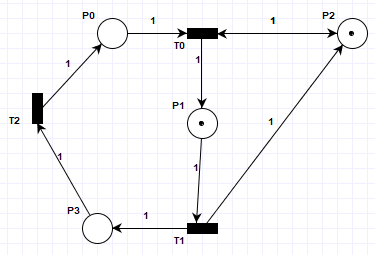
\includegraphics[width=10cm]{lab6/n1.png}
            \caption{Projekt sieci z zadania pierwszego}
        \end{figure}\\
        Następnie przeprowadziłem analizę niezmienników, otrzymując następujące wyniki.
        \begin{figure}[h!]
            \centering
            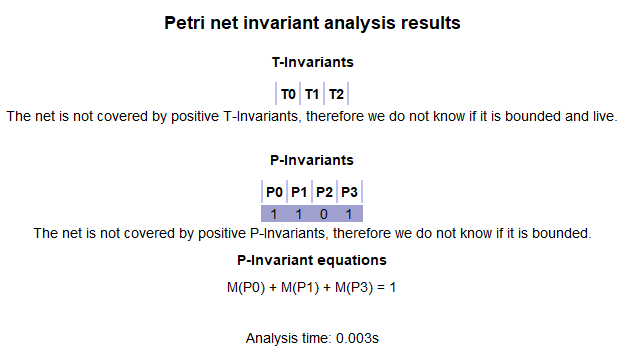
\includegraphics[width=14cm]{lab6/n1_1.png}
            \caption{Analiza niezmienników sieci z zadania pierwszego}
        \end{figure}\\
        Na ich podstawie wywnioskować możemy, że sieć nie jest odwracalna, tzn nie istnieje wektor będący T-niezmiennikiem przejść. 
        Wygenerowałem także graf osiągalności dla sieci.
        \begin{figure}[h!]
            \centering
            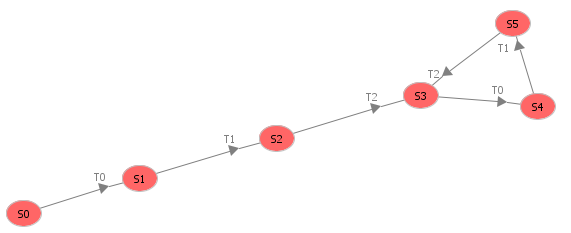
\includegraphics[width=14cm]{lab6/n1_2.png}
            \caption{Graf osiągalności sieci z zadania pierwszego}
        \end{figure}\\
        Sieć jest żywa, jeśli ze znakowania początkowego możemy wykonać dowolne przejście jako pewną sekwencję przejść. Na podstawie wygenerowanego grafu, oraz powyższej definicji wywnioskować możemy, że otrzymana sieć jest żywa. \\
        Sieć nie jest ograniczona, ponieważ w stanie S4 ilość znaczników nie jest ograniczona.
        \begin{figure}[h!]
            \centering
            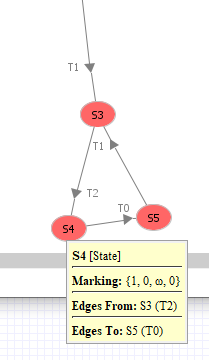
\includegraphics[width=7cm]{lab6/n1_3.png}
            \caption{Graf osiągalności sieci z zadania pierwszego, znaczniki stanu czwartego}
        \end{figure}\\

    \newpage
    \section{Zadanie 2}
        Przeprowadziłem symulację problemu producenta-konsumenta z ograniczonym buforem (sieć przykładowa programu).
        \begin{figure}[h!]
            \centering
            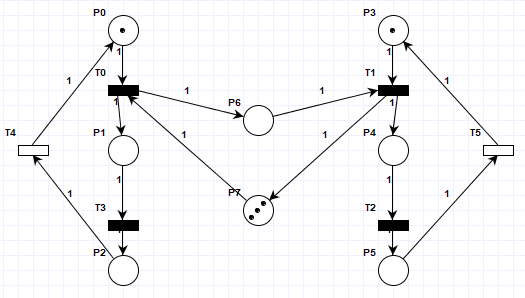
\includegraphics[width=10cm]{lab6/n2.png}
            \caption{Projekt sieci z zadania drugiego}
        \end{figure}\\
        Przeprowadziłem analizę niezmienników.
        \begin{figure}[h!]
            \centering
            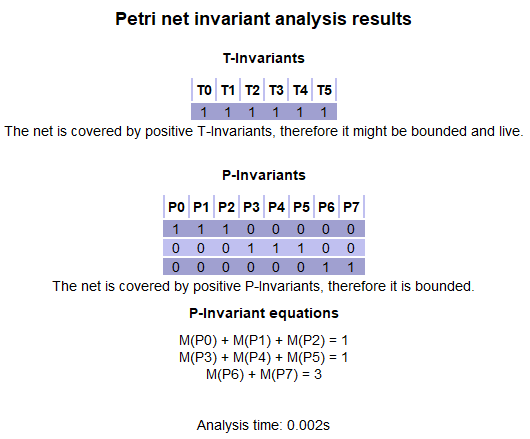
\includegraphics[width=10cm]{lab6/n2_1.png}
            \caption{Analiza niezmienników sieci z zadania drugiego}
        \end{figure}\\
        O rozmiarze bufora mówi nam ostatnie równanie, tj. $M(P6) + M(P7) = 3$, ma on zatem rozmiar trzech elementów.
        Sieć jest zachowawcza, ponieważ liczba znaczników w każdym znakowaniu osiągalnym ze znakowania początkowego jest taka sama.

    \newpage
    \section{Zadanie 3}
        W symulatorze przygotowałem sieć reprezentującą problem producenta-konsumenta z nieograniczonym buforem według poniższego projektu.
        \begin{figure}[h!]
            \centering
            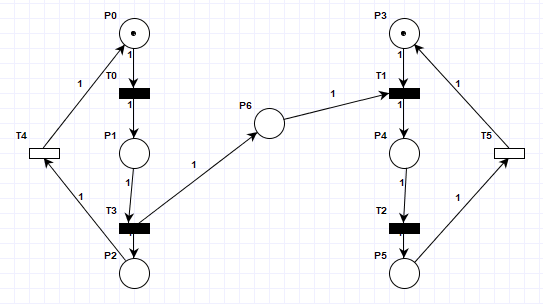
\includegraphics[width=10cm]{lab6/n3.png}
            \caption{Projekt sieci z zadania trzeciego}
        \end{figure}\\
        \FloatBarrier
        Przeprowadziłem analizę niezmienników. 
        \begin{figure}[h!]
            \centering
            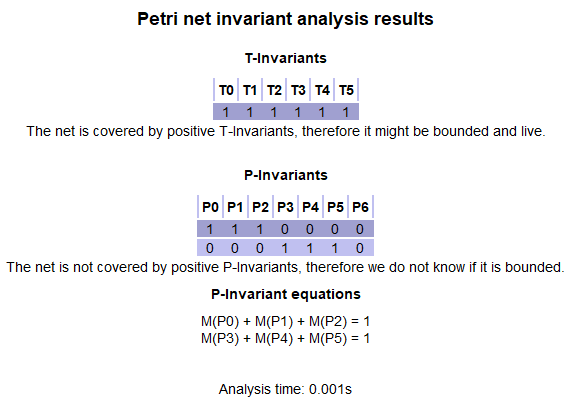
\includegraphics[width=10cm]{lab6/n3_1.png}
            \caption{Analiza niezmienników sieci z zadania trzeciego}
        \end{figure}\\
        \FloatBarrier
        Sieć cechuje brak pełnego pokrycia miejsc. 
    
    \newpage
    \section{Zadanie 4}
        W symulatorze przygotowałem sieć ze wzajemnym wykluczaniem dwóch procesów na wspólnym zasobie według poniższego projektu.
        \begin{figure}[h!]
            \centering
            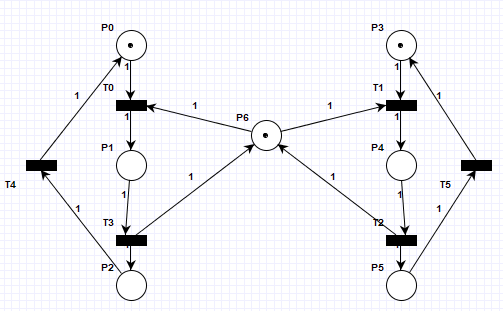
\includegraphics[width=10cm]{lab6/n4.png}
            \caption{Projekt sieci z zadania czwartego}
        \end{figure}\\
        \FloatBarrier
        Przeprowadziłem analizę niezmienników. 
        \begin{figure}[h!]
            \centering
            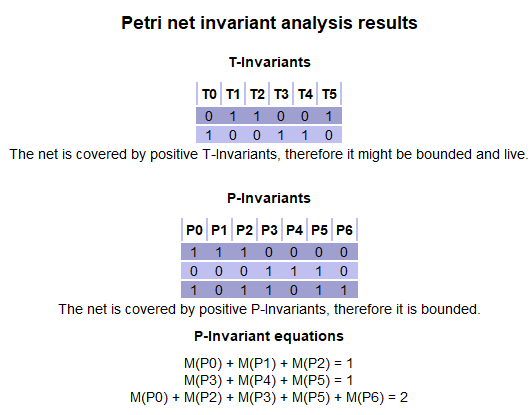
\includegraphics[width=10cm]{lab6/n4_1.png}
            \caption{Analiza niezmienników sieci z zadania czwartego}
        \end{figure}\\

    \newpage
    \section{Zadanie 5}
        W symulatorze przygotowałem sieć z zakleszczeniem według poniższego projektu.
        \begin{figure}[h!]
            \centering
            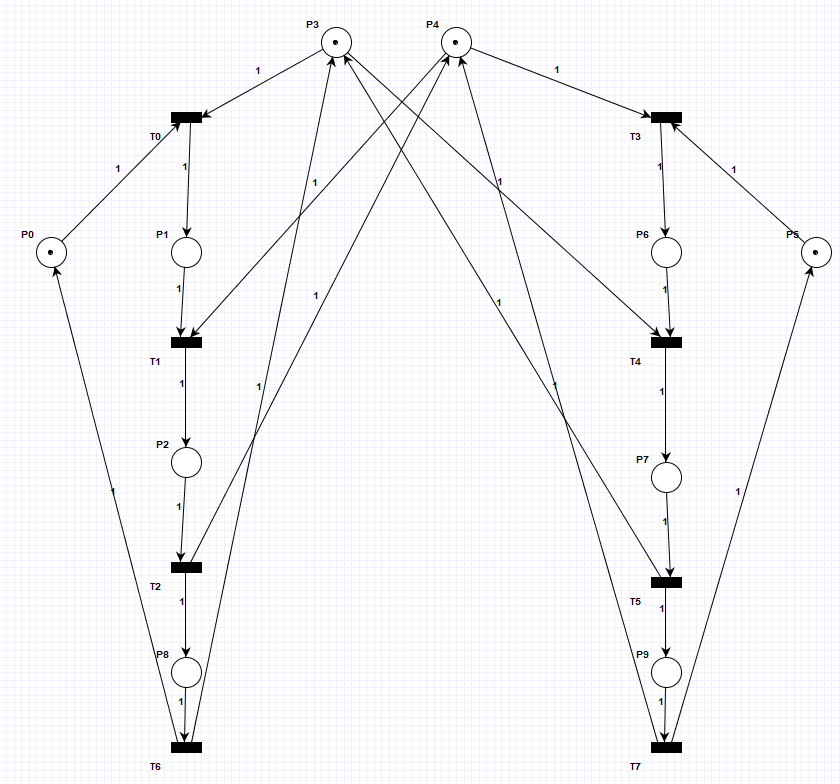
\includegraphics[width=10cm]{lab6/n5.png}
            \caption{Projekt sieci z zadania piątego}
        \end{figure}\\
        Wygenerowałem graf osiągalności. 
        \begin{figure}[h!]
            \centering
            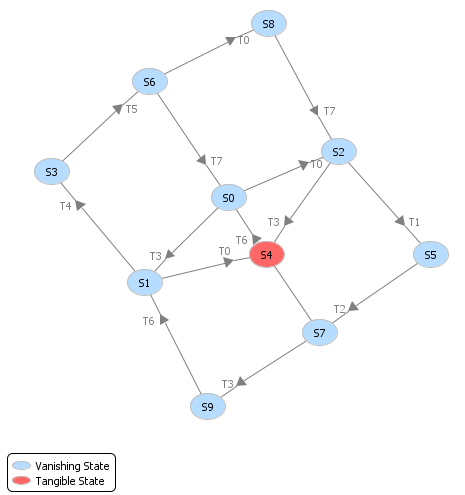
\includegraphics[width=10cm]{lab6/n5_1.png}
            \caption{Analiza niezmienników sieci z zadania piątego}
        \end{figure}\\

        
\end{document}

% \begin{figure}[h!]
%     \centering
%     \includegraphics[width=13cm]{reports/img/Z1A_polpelny.png}
%     \caption{Sumator pół-pełny}
% \end{figure}\\
